\bigskip 
\bigskip 
\subsubsection{Contenido}
\bigskip 
%\begin{wrapfigure}{r}{0.5\textwidth}
%  \begin{center}
%    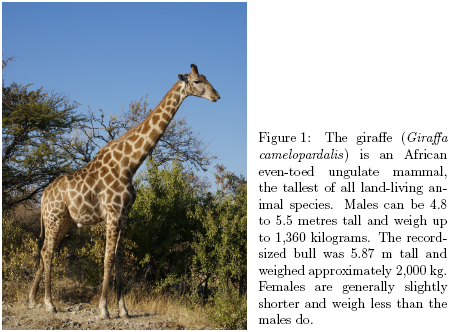
\includegraphics[width=0.48\textwidth]{./ingles/Latex_example_sidecap.jpg}
%  \end{center}
%\end{wrapfigure}

\begin{description}
\item[Nombre:] Balalaika
\item[Cristaleria:] Vaso largo (10oz / 300cc)
\item[M\'etodo de elaboraci\'on:] Batido
\item[Decoraci\'on:] Sin decoraci\'on.
\end{description}

\begin{table}[h]
\caption{Ingredientes y proporciones} 
\label{tab:fonts}
\begin{center}       
\begin{tabular}{|l|l|l|c|l|} %% this creates two columns
%% |l|l| to left justify each column entry
%% |c|c| to center each column entry
%% use of \rule[]{}{} below opens up each row
\hline
\rule[-1ex]{0pt}{3.5ex}  \textbf{Producto} & \textbf{Bebida} & \textbf{Marca} & \textbf{Volumen} & \textbf{Fraccion}  \\
\hline
\rule[-1ex]{0pt}{3.5ex}  Aguardiente & Vodka 			& Wyborowa 		& 2 oz / 60 cc 	&  	\\
\hline
\rule[-1ex]{0pt}{3.5ex}  Licor 		& Triple Sec 	& Cointreau 				& 1 1/2 oz / 45 cc 		&  	\\
\hline
\rule[-1ex]{0pt}{3.5ex}  Fruta 		& Limon & Jugo	& 1 1/2 oz / 45 cc		& 	\\
\hline

\end{tabular}
\end{center}
\end{table} 
\bigskip 

%%-----------------------------------------------------------
\subsubsection{Formato de elaboraci\'on} 
\label{sec:title}
\bigskip 
\begin{center}
\begin{enumerate}
\item Colocar en una coctelera una pala de hielo.
\item Servir los ingredientes en la misma.
\item Batir hasta que la coctelera est\'e helada.
\item Servir sin filtro en el vaso de trago largo.

\end{enumerate}
\end{center}
\bigskip 
\bigskip 
%%%%%%%%%%%%%%%%%%%%%%%%%%%%%%%%%%%%%%%%%%%%%%%%%%%%%%%%%%%%%

\subsubsection{Notas}
\bigskip 
\begin{center}
\raggedright{}Servir con sorbete.
\end{center} 

%\subsubsection{Informaci\'on extra}
\bigskip
%\begin{center}
\medskip 
%\raggedright{ \textbf{Or\'igenes de este trago}} \\ 
\medskip


%\end{center}